\documentclass[18pt]{article}
\usepackage[utf8]{inputenc}
\usepackage[T1]{fontenc}
\usepackage{ragged2e}
\usepackage{caladea}
\usepackage{graphicx}
\usepackage{longtable}
\usepackage{wrapfig}
\usepackage{rotating}
\usepackage{epigraph}
\usepackage[normalem]{ulem}
\usepackage{hyperref}
\usepackage{amsmath}
\usepackage{amssymb}
\usepackage{capt-of}
\usepackage{hyperref}
\usepackage{fancyhdr}
\usepackage{verse}

\title{
 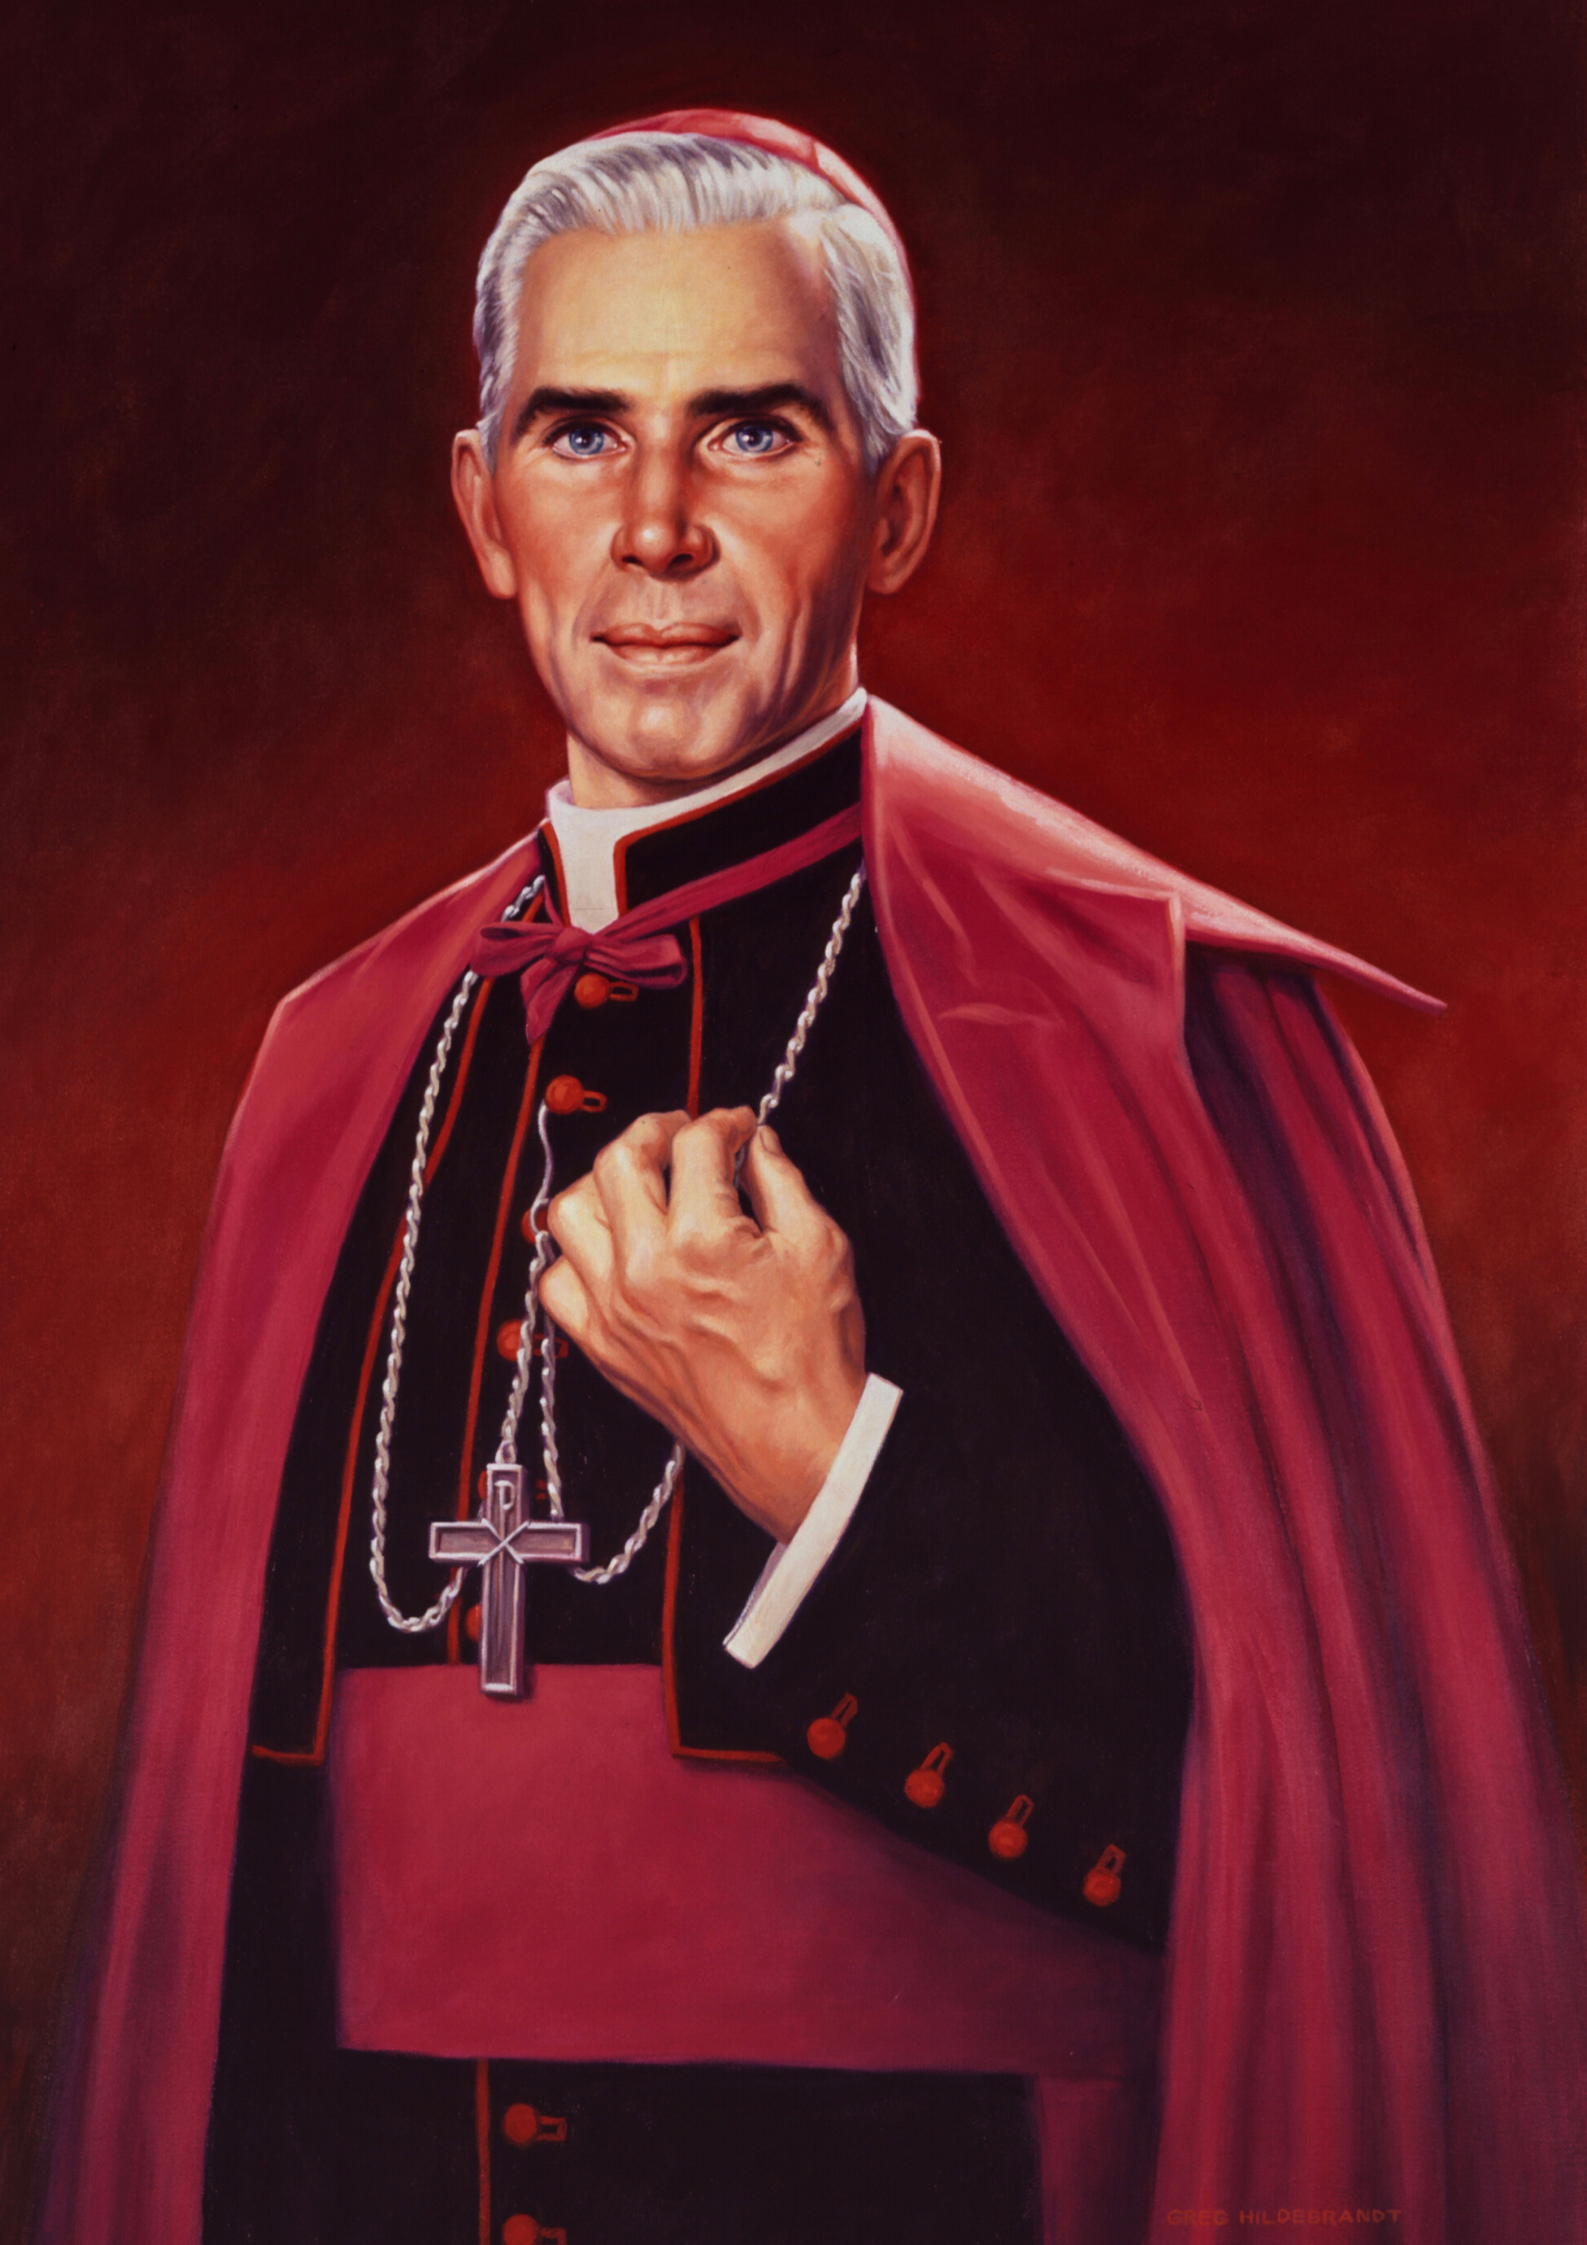
\includegraphics[scale=.4, trim={10cm, 0, 10cm, 0}]{./assets/imagem.jpg}
  \par
   NOVENA A SÃO CIRILO DE JERUSALÉM}
  \date{Início da Novena : 09/03 - Data Litúrgica: 18/03} 
  \author{Garamog, Nina Freitas}


% Comando para fazer "Sumário" não aparecer no Sumário.
\renewcommand{\contentsname}{Sumário}

\begin{document}

\thispagestyle{empty} %zera a primeira página

\maketitle

\newpage
\tableofcontents


\pagestyle{fancy}
\fancyhf{} % clear existing header/footer entries
\fancyfoot[LO, CE]{
\includegraphics[scale=0.2]{./assets/cross.png} São São Cirilo de Jerusalém, rogai por nós! }
% Place Page X of Y on the right-hand
% side of the footer
\fancyfoot[R]{\thepage}

\centering
\vfill
Visite-nos no Telegram: \url{https://t.me/CotidieNovena}

\newpage
%%%%%%%%%%%%%%%%%%%%%%%%%%%%%%%%%%%% História %%%%%%%%%%%%%%%%%%%%%%%%%%%%%%%%%%%%%%%%%%


\begin{justify}
 \section{História}


 \begin{justify}
  \subsection{Origens}
 \end{justify}

São Cirilo de Jerusalém nasceu por volta do ano de 315 em Jerusalém ou em seus arredores. Pouco se sabe sobre sua infância e juventude, além de que ele cresceu num lar cristão, com uma vida financeira confortável. Recebeu uma sólida formação nas Sagradas Escrituras e em matérias humanísticas.

 \begin{justify}
  \subsection{Sacerdote aos 30 anos}
 \end{justify}

Ordenado sacerdote em 345, aos 30 anos, ele foi sagrado bispo de Jerusalém apenas três anos mais tarde, em 348. São Cirilo de Jerusalém viveu numa época em que a Igreja do Oriente estava envolvida em muitas controvérsias.  São Cirilo precisou enfrentar especialmente a heresia do arianismo. O arianismo basicamente negava a consubstancialidade entre Jesus e Deus Pai, ou seja, segundo os arianos, Jesus seria o filho de Deus, mas não o próprio Deus.

 \begin{justify}
  \subsection{Escritos valiosos}
 \end{justify}

São Cirilo deixou para a Tradição da Igreja diversos escritos, mas os mais famosos deles são as suas 24 catequeses, que estão entre os mais preciosos tesouros da antiguidade cristã. Suas catequeses foram escritas como parte da preparação dos catecúmenos para o batismo. Nela, incluem uma introdução, dezoito catequeses aplicadas durante a Quaresma e cinco “catequeses mistagógicas”, que foram ministradas durante a semana de Páscoa para aqueles mesmos que receberam o batismo.

 \begin{justify}
  \subsection{Catequeses}
 \end{justify}


As catequeses são marcadas pelo rigor em relação à doutrina. A grande habilidade de São Cirilo em explicar conceitos complexos de forma simples e direta, facilita o entendimento. A título exemplificativo, vejamos como ele explica o significado da proclamação “Corações ao alto!”, na quinta catequese mistagógica:

“Verdadeiramente, nesta hora mui tremenda, é preciso ter o coração no alto, junto de Deus, e não embaixo, na terra, nas coisas terrenas. Com autoridade, pois, o sacerdote ordena que, nesta hora, se abandonem todas as preocupações da vida e os cuidados domésticos e que se tenha o coração no céu, junto ao Deus benevolente.”

 \begin{justify}
  \subsection{O capítulo das perseguições}
 \end{justify}

A vida de São Cirilo não se resumiu às suas brilhantes catequeses, ela foi também marcada por polêmicas e perseguições justamente por causa do arianismo. Acácio, um bispo muito influente na época, simpatizante do arianismo, teria nomeado São Cirilo bispo de Jerusalém imaginando que fosse tê-lo como aliado na defesa da heresia. Mantendo-se fiel à sã doutrina, São Cirilo foi perseguido e acabou enfrentando por três vezes o exílio. A primeira vez em 357, conforme disposto por um Sínodo em Jerusalém. A segunda em 360, por obra direta de Acácio. O último exílio foi em 367, o seu mais longo exílio, que durou 11 anos, por obra direta do imperador Valente, que também era ariano. 

Com a morte do imperador, em 378, São Cirilo pôde finalmente voltar para a sua sede episcopal em ânimo definitivo. Participou em 381, do Concílio Ecumênico de Constantinopla, onde foi firmado o símbolo Niceno-Constatinopolitano.
Proclamado Doutor da Igreja e o seu reflexo na atualidade

 \begin{justify}
  \subsection{Páscoa}
 \end{justify}

Em 386, provavelmente no dia 18 de março, São Cirilo morreu, aos 71 anos de idade. Em meio a muitas acusações de heresia, São Cirilo permaneceu fiel à Igreja de Cristo. Foi paciente nas perseguições e sua ortodoxia foi reconhecida a tal ponto que em 1882 o Papa Leão XIII o proclamou Doutor da Igreja. 

 \begin{justify}
  \subsection{Fontes de documentos atuais}
 \end{justify}

Além disso, duas importantes constituições dogmáticas do Concílio Vaticano II, a Lumen Gentium e a Dei Verbum, foram inspiradas em seus escritos.

 \begin{justify}
  \subsection{Sua repercussão na atualidade}
 \end{justify}

São Cirilo de Jerusalém ajuda, até hoje, cristãos de todo o mundo a mergulharem no mistério da fé, como tão bem expressou o Papa Bento XVI:

O mistério que se deve desvendar é o desígnio de Deus, que se realiza através das ações salvíficas de Cristo na Igreja. Por sua vez, a dimensão mistagógica está acompanhada pela dos símbolos, que expressam a vivência espiritual que eles fazem “explodir”. Assim, a catequese de Cirilo, com base nas três componentes descritas – doutrinal, moral e, por fim, mistagógica –, resulta numa catequese global no Espírito. A dimensão mistagógica atua como síntese das duas primeiras, orientando-as para a celebração sacramental, na qual se realiza a salvação do homem todo. Trata-se, em definitivo, de uma catequese integral, que envolvendo corpo, alma e espírito permanece emblemática também para a formação catequética dos cristãos de hoje.

 \begin{justify}
  \subsection{Ação de Deus}
 \end{justify}

Olhando para a vida de São Cirilo, encanta-nos o que o Espírito Santo pode realizar na vida de quem se abre à graça de Deus: de um lado, um dom impressionante para transmitir a fé e a sã doutrina, por meio de catequeses que continuam atualíssimas até hoje; do outro lado, a paciência e a fortaleza para viver perseguido e não se render, não ceder ao desânimo nem ao cansaço. Mesmo que, imitando a Cristo, por tanto tempo não tenha tido um lugar onde reclinar a cabeça.


\vfill

\href{https://santo.cancaonova.com/santo/sao-cirilo-de-jerusalem/}{Fonte: Canção Nova}

\end{justify}

%%%%%%%%%%%%%%%%%%%%%%%%%%%%%%%%%%%%% Orações %%%%%%%%%%%%%%%%%%%%%%%%%%%%%%%%%%%%%%%%%%%
\begin{justify}

\newpage
\begin{center}
 \section{Orações}\label{sec:Orações} % (fold)
\textit{Em nome do Pai, e do Filho, e do Espírito Santo. Amém.}
\end{center}

\subsection{Oração Inicial}

\textbf{Mãe de Deus}

 \settowidth{\versewidth}{Salve, Maria, Mãe de Deus,}
Salve, Maria, Mãe de Deus,  
precioso tesouro de todo o universo,  
lâmpada que nunca se apaga, coroa de virgindade,  
sustento da verdadeira fé, templo indestrutível,  
morada d'Aquele que nenhum lugar pode conter,  
Ó Mãe e Virgem.  
Por meio de você, todos os santos Evangelhos chamam bendito  
Aquele que vem em nome do Senhor.

Salve, Mãe de Deus.  
Você encerrou em seu coração o Deus infinito  
que nenhum espaço pode conter.  
Por meio de você, a Santíssima Trindade é adorada e glorificada,  
a preciosa cruz é venerada em todo o universo.  
Por meio de você, os céus se alegram,  
e os anjos e arcanjos se enchem de alegria.  
Por meio de você, os demônios são banidos,  
e o tentador caiu do céu.  
Por meio de você, a raça humana caída é admitida no céu.

Salve, Mãe de Deus.  
Por meio de você, os reis governam,  
e o Filho unigênito de Deus se tornou uma estrela de luz  
para aqueles que estavam sentados em trevas  
e na sombra da morte.


\subsection{Oração de Todos os Dias}


Ó Deus, que fizeste do Bispo São Cirilo de Alexandria  
um campeão invencível da divina maternidade  
da Santíssima Virgem Maria,  
concede, nós te pedimos, que nós,  
que acreditamos que ela é verdadeiramente a Mãe de Deus,  
sejamos salvos pela Encarnação de Cristo, Teu Filho,  
que vive e reina contigo  
na unidade do Espírito Santo,  
um só Deus, para sempre.

Lembra-te, ó Pai Todo-Poderoso, do momento em que,  
de acordo com a Tua vontade,  
a “plenitude do tempo” chegou para estes povos e nações.  
Quando estes santos Missionários,  
Santos Cirilo e Metódio,  
cumpriram fielmente o mandamento que Teu Filho, Jesus Cristo,  
confiou aos Seus Apóstolos;  
seguindo os seus passos,  
trouxeram às terras habitadas pelos eslavos  
a luz do Evangelho, a Fé Católica.

Ó Senhor, concede nossos pedidos pessoais,  
(mencione em silêncio sua necessidade pessoal)  
e através desta Novena,  
que possamos construir sobre a fé de muitos  
de nossas famílias imigrantes da Checoslováquia,  
rezar com o Venerável João Paulo II,  
o Papa de origem eslava,  
e receber Tuas graças e favores.

Pela intercessão de São Cirilo e São Metódio,  
que Deus conceda que nós, de muitas ascendências,  
continuemos a obra de Cristo através de Sua Igreja,  
em nossas vidas, nossas famílias e todos os povos  
e que tenhamos força para superar todo ódio  
e conquistar todo o mal com o bem.




\begin{center}
\textbf{\textit{Pai Nosso, Ave Maria e Glória ao Pai.}}
\end{center}

\vfill

\begin{center}
\section*{São Cirilo de Jerusalém, Rogai por nós!}
\end{center}

\href{https://www.catholicdoors.com/prayers/novenas/p03972.htm}{Fonte: Catholic Outdoor}

\vfill


\end{justify}

\end{document}
